\documentclass{article}
% --- watermark (auto-inserted) ---
\usepackage{xcolor}
\usepackage{xfp}% \fpeval; in the kernel since 2022, harmless on older LaTeX
\usepackage{draftwatermark}
\newlength{\watermarkTextWidth}
\AddToHook{begindocument/end}{%
  \SetWatermarkText{\normalfont Generated by The Agentic Scientist}%
  \SetWatermarkFontSize{10pt}%
  \SetWatermarkLightness{0.85}%
  \settowidth{\watermarkTextWidth}{\normalfont\fontsize{10pt}{12pt}\selectfont Generated by The Agentic Scientist}%
  \edef\watermarkScale{\fpeval{0.8 * sqrt(\paperwidth**2 + \paperheight**2) / \watermarkTextWidth}}%
  \edef\watermarkAngle{\fpeval{atand(\paperheight/\paperwidth)}}%
  \SetWatermarkScale{\watermarkScale}%
  \SetWatermarkAngle{\watermarkAngle}%
}
% --- end watermark ---

\usepackage{iclr2026_conference,times}
\usepackage{amsmath,amssymb,booktabs,graphicx,longtable,subcaption}
\usepackage{hyperref,url}
\title{Protected Reporting After Prompt Selection:\\Benefits and Limits}

\begin{document}
\maketitle

\begin{abstract}
Selecting a prompt on benchmark questions and reporting its selection score confounds performance with favorable sampling noise. Reserving questions for reporting removes this direct reuse, but sacrifices observations and may change which prompt is selected. We examine that trade-off with a frozen prompt bank, known-truth simulations, and genuine CPU inference on MMLU-Pro. The controlled comparison holds the selected prompt fixed and changes only the observations used to report its score. Across five evaluation seeds, protected half-split reporting reduces mean squared error relative to selection-score reuse by 43--46\% in the sixteen-prompt simulations and reduces squared discrepancy to a separate real-model audit by 54--76\%. These benefits are not universal: full-budget reuse has lower mean error in every synthetic condition, and reporting error does not establish better selected-prompt accuracy. Real-model comparisons use finite audits, not known population accuracy. The evidence supports reporting target, sample allocation, and audit uncertainty as necessary parts of interpreting an optimized benchmark score, rather than endorsing a uniformly superior estimator.
% @evidence[[analysis/summary.json#/reductions_percent]]
% @evidence[[paper_data.json#/final_evaluation/evaluation_evidence/episodes]]
\end{abstract}

\section{Introduction}
An optimized benchmark score answers a different question from an independently measured score. When a system chooses among prompt configurations using a finite question set, the selected configuration benefits both from its underlying quality and from the noise that favored it on those questions. Repeating the selected score as the performance estimate leaves those contributions entangled. This matters even when the model weights are unchanged, the prompt bank is fixed, and every answer is evaluated consistently.

A conventional response is to reserve questions that do not participate in selection. Yet that prescription alone does not settle how a reported score should be interpreted. Holding out questions reduces the sample available to select a prompt and the sample available to estimate its performance. A no-search configuration can therefore have lower estimation error while being a less accurate system. Conversely, a selected configuration can have a more trustworthy report without becoming more accurate. Any empirical comparison must state which prompt is being evaluated, which observations chose it, and what reference defines estimation error.

This paper asks: \emph{when does protected reporting reduce error after prompt selection, and what does an independent finite audit establish about that reduction?} We study a frozen bank with randomized half-split selection and reporting. The primary baseline reports the selection score of the \emph{same} selected prompt. This isolates the reporting-data contrast from changes in the selected system. Additional baselines expose the cost of protection: full-budget selection and reuse, all-question fixed and random prompts, and an alternative half split.

The empirical contribution is deliberately bounded. Known-truth simulations separate selection optimism, reporting bias, squared error, and interval coverage. Real answer generation supplies a benchmark check, while an explicit distinction between finite-audit agreement and population accuracy prevents that check from being overinterpreted. The results show substantial improvements over same-winner reuse when selecting among sixteen prompts, but also clear counterexamples to universal error reduction. The study evaluates a conventional reporting design rather than proposing a new optimizer or a new post-selection guarantee.
% @evidence[[paper_data.json#/final_evaluation/evaluation_evidence/episodes]]

\begin{figure}[t]
\centering

\includegraphics[width=\textwidth]{figures/reporting_overview.png}
\caption{Selection and reporting have different data roles. The protected and reuse reports describe the same selected prompt; full-budget selection can choose another prompt. Known truth supports population-error measurements in simulation, whereas a separate real-model audit supplies a noisy finite reference. Protection is an intended partition property, not a claim that every source of benchmark dependence has been eliminated.}
\label{fig:overview}
\end{figure}

\section{Related Work}
\paragraph{Selection and assessment.}
Separating model choice from assessment is classical \citep{Stone1974CrossValidation,Arlot2010Survey}. Optimization of a noisy selection criterion can bias the resulting performance estimate \citep{Cawley2010Overfitting,Varma2006Bias}. Feature-selection studies provide another setting in which assessment must encompass the selection operation \citep{Ambroise2002Selection,Guyon2003Selection}. Our prompt-selection setting is simpler than learned feature selection, but shares the distinction between a fixed estimator and an estimator chosen using the assessment data. Cross-validation itself has multiple possible targets; its uncertainty is not determined by the number of reported splits alone \citep{Bates2021CrossValidation,Bengio2004Variance,Varoquaux2018CrossValidation}.

\paragraph{Prompts and benchmarks.}
Prompt sensitivity motivates examining a bank rather than treating a single wording as intrinsic to a model \citep{Sclar2024Formatting}. Multi-prompt evaluation estimates performance across prompt variants \citep{Polo2024MultiPrompt}; budgeted best-arm identification instead concerns choosing a strong prompt \citep{Shi2024BestArm}. We address the report attached to the chosen prompt, not either procedure's optimization efficiency. MMLU-Pro supplies the real multiple-choice setting \citep{Wang2024MMLUPro}; this study does not reproduce the benchmark paper's model comparisons.

\paragraph{Inference after selection.}
Winner inference and post-selection inference formalize why a data-dependent target complicates conventional uncertainty statements \citep{Andrews2018Winners,Berk2013PostSelection}. Adaptive data analysis and reliable leaderboards consider repeated feedback from shared data \citep{Dwork2015Adaptive,Blum2015Ladder}; our frozen, noninteractive bank does not test those guarantees. Simultaneous approximations for maxima address another inferential route \citep{Chernozhukov2013Gaussian}, which is not implemented here. The distinction between controlling an error criterion and estimating a system's accuracy also appears in multiple testing \citep{Benjamini1995}.

\paragraph{Uncertainty and comparisons.}
Binomial interval behavior depends on the construction and sampling regime \citep{Brown2001Binomial}. Resampling can estimate uncertainty, but bootstrap methodology does not automatically validate an arbitrary resampling unit \citep{Efron1979Bootstrap,DiCiccio1996Bootstrap}. Method-comparison literature emphasizes the evaluation unit and dependence structure \citep{Dietterich1998Tests,Nadeau2003Inference,Demsar2006Comparisons}. Accordingly, we show seed-level variation without treating overlapping benchmark samples as independent datasets or presenting an unperformed significance test.

\section{Method}
\subsection{Problem Setup and Reporting Targets}
Let $X_{ij}\in\{0,1\}$ indicate whether prompt $j$ answers question $i$ accurately. There are $n$ available questions and $K$ prompt configurations. The objective of selection is high answer accuracy, whereas the objective of reporting is low estimation error for the selected configuration. A seeded random partition creates disjoint sets $S$ and $R$, with $|S|=|R|=n/2$. Define
\begin{equation}
 \widehat j=\arg\max_{j\in\{1,\ldots,K\}}\overline X_{Sj},\qquad
 \widehat p_{\rm reuse}=\overline X_{S\widehat j},\qquad
 \widehat p_{\rm protect}=\overline X_{R\widehat j}.
 \label{eq:estimators}
\end{equation}
Ties follow the fixed order of the prompt bank. Both reports in Equation~\ref{eq:estimators} concern precisely the same configuration. A smaller error for the protected report therefore cannot be interpreted as an increase in that configuration's accuracy.
% @evidence[[source_evidence/downstream/program/src/program.py#L97]]
% @evidence[[source_evidence/evaluate_final.py#L753]]

In simulation, the reference $p_j$ is the generating marginal accuracy. We measure $(\widehat p-p_{\widehat j})^2$, reporting bias $\widehat p_{\rm protect}-p_{\widehat j}$, and selection optimism $\widehat p_{\rm reuse}-p_{\widehat j}$. In the real-model setting, $p_j$ is unavailable. We instead use the observed accuracy $\widehat a_j$ on a separate audit set, and measure $(\widehat p-\widehat a_{\widehat j})^2$. We call the latter \emph{audit-reference error}. It includes noise in the audit reference and is not a directly observed population MSE.
% @evidence[[source_evidence/evaluate_final.py#L760]]
% @evidence[[source_evidence/evaluate_final.py#L969]]

\subsection{Design Rationale and Compared Approaches}
The rationale for protection is that observations which select $\widehat j$ should not also determine its report. Under independent, identically distributed question sampling and a bank fixed independently of the report data, reporting on fresh observations avoids the direct maximization of report noise. These assumptions explain the design; they are not themselves established by passing implementation checks. Within a finite shared question pool, disjointness alone does not supply a general population theorem.

The primary comparison changes the reporting rows in Equation~\ref{eq:estimators}, not the selected prompt or the total question set. It is not a comparison with selecting on all questions. To expose that distinction, \emph{full reuse} selects the highest-scoring prompt on all $n$ rows and reports that same all-row score. Its reference is the accuracy of \emph{its own} selected prompt. The \emph{fixed} comparator reports the all-row accuracy of the default prompt. The \emph{random} comparator chooses a seeded prompt index and reports its all-row accuracy. Both use their own prompt's reference, not $p_{\widehat j}$.

An \emph{alternative half split} selects on the first half of the supplied rows and reports on the second half. This is another protected design, not an independent methodological innovation. Because it can select a different prompt, its comparison with the randomized split is not a pure reporting-data ablation. Likewise, contrasts with fixed, random, and full-reuse configurations jointly change the sample allocation or the selected system. We retain them to reveal practical trade-offs, not to attribute every difference causally to protection.
% @evidence[[source_evidence/evaluate_final.py#L760]]

The reported interval is the usual 95\% Wilson score interval evaluated on $|R|$ Bernoulli observations. Its coverage is measured against known truth only in simulation. On real questions, the same containment indicator checks whether the interval includes the audit accuracy. These are different diagnostics. Interval width is on the accuracy scale, not an uncertainty interval for the MSE comparison.
% @evidence[[source_evidence/evaluate_final.py#L746]]

\subsection{Experimental Protocol}
The completed evaluation contains seeds $1009,2027,3037,4051,5059$. Each seed covers synthetic and real conditions with $n\in\{64,256\}$ and $K\in\{1,16\}$. Thus each seed contributes eight conditions; the single-prompt conditions remove selection multiplicity without changing the reporting rule. Synthetic conditions average four regimes, each with $1024$ independently generated matrices. Real conditions contain one realized selection/report/audit comparison per seed, not thousands of repeated model fits.
% @evidence[[paper_data.json#/final_evaluation/evaluation_evidence/episodes]]
% @evidence[[source_evidence/evaluate_final.py#L899]]

All descriptive condition means give seeds equal weight. Within a synthetic condition, regimes and replicates have equal weight. The overall summary gives the two evidence families and their question/prompt settings equal weight; it does not pool real audit questions with individual synthetic replicates. Figures show the actual seed observations, rather than confidence bars reconstructed from marginal MSE standard errors. We make no across-seed significance claim. The available summaries do not retain paired replicate-level error differences needed for such a comparison.

The studied policy is the retained baseline, not an improved configuration discovered by the search. Three alternative allocations produced no usable scored evaluations and cannot be treated as measured losses or successful ablations. The independent final evaluation completed with a qualified outcome. This records protocol qualification, not superiority, novel methodology, or complete evidence of external validity. Diagnostic records attributed to the candidate remain unverified, and absent detailed gate diagnostics remain unknown.
% @evidence[[paper_data.json#/downstream_study]]
% @evidence[[paper_data.json#/final_evaluation/status]]
% @evidence[[paper_data.json#/final_evaluation/outcome]]
% @evidence[[paper_data.json#/final_evaluation/evaluation_evidence/candidate_diagnostics_trust]]

\subsection{Known-Truth Construction}
The four synthetic regimes cross equal versus graded marginal prompt accuracies with low versus high shared-outcome coupling. Equal accuracies are $p_j=0.6$. Graded accuracies are equally spaced from $0.4$ to $0.8$; for $K=1$ the implementation uses $p_1=0.4$. Let $U_0,U_1,\ldots,U_K$ be independent uniforms for each question and let $c\in\{0.1,0.9\}$. The implemented construction is
\begin{equation}
 V_j=\begin{cases}U_0/c,&U_0<c,\\ U_j,&U_0\geq c,\end{cases}
 \qquad X_j=\mathbf{1}\{V_j<p_j\}.
 \label{eq:synthetic}
\end{equation}
The shared branch changes prompt-outcome dependence while preserving marginal accuracy. We call $c$ a coupling probability, not the exact Pearson correlation for every pair of unequal-accuracy prompts. Every matrix is generated from its seed, size, prompt count, and regime; the evaluator checks the raw uniform draws against retained hashes. This construction permits population-error and coverage measurements but does not model the full dependence or difficulty structure of natural benchmark questions.
% @evidence[[source_evidence/evaluate_final.py#L938]]
% @evidence[[paper_data.json#/final_evaluation/evaluation_evidence/episodes/0/solution/cases/0/details]]

\subsection{Real Inference and Implementation}
The real condition uses \texttt{HuggingFaceTB/SmolLM2-135M-Instruct} on CPU in float32 with MMLU-Pro. Model and dataset revisions are fixed and recorded in Supplementary Information. The prompt bank contains sixteen frozen, short instructions asking for a choice letter. The $K=1$ condition uses only the default instruction; $K=16$ uses the full bank. A reset-seeded shuffle partitions supplied question keys, reporting weights are uniform, and tie priority follows bank order. The policy receives question identifiers and subject strata, but not answer observations; it does not adapt the bank using within-evaluation feedback.
% @evidence[[source_evidence/resources/runtime_manifest.json]]
% @evidence[[source_evidence/resources/split_manifest.json]]
% @evidence[[source_evidence/downstream/program/src/program.py#L70]]

For each seed, the evaluator samples $n+512$ questions without replacement from its retained pool; the final $512$ form the audit. The benchmark subset and audit are disjoint within a condition. Samples overlap across conditions and seeds, so this design does not create independent benchmark replications. Normalized question stems and normalized question/option content are checked for split overlap. These checks do not exclude pretraining exposure or all semantic duplicates.
% @evidence[[source_evidence/evaluate_final.py#L694]]
% @evidence[[source_evidence/evaluate_final.py#L912]]
% @evidence[[paper_data.json#/final_evaluation/evaluation_evidence/episodes]]

Answer generation applies the model's chat template and deterministically chooses one token constrained to legal answer letters. Inputs longer than $2044$ tokens and invalid responses count as errors; they are not silently omitted. Batches contain up to eight inputs, and a question-content/prompt cache reuses outputs. This is direct constrained answering, not free-form reasoning. The inference worker fixes its tensor seed and uses deterministic operations. The small model and decoding restriction are part of the evaluated configuration and limit transfer to larger or reasoning-capable systems.
% @evidence[[source_evidence/evaluate_final.py#L574]]

For selected-versus-default accuracy, the evaluator resamples audit subjects with replacement, retaining all paired question outcomes within each sampled subject. It takes percentile endpoints from $200$ bootstrap draws. These descriptive 95\% intervals are neither simultaneous across settings nor a validation of the bootstrap's sampling properties. They address an accuracy difference, not the error of the protected report.
% @evidence[[source_evidence/evaluate_final.py#L987]]
% @evidence[[paper_data.json#/final_evaluation/evaluation_evidence/episodes]]

\section{Results}
\subsection{Reporting Error Depends on the Comparator}
Figure~\ref{fig:errors} separates known-truth MSE from audit-reference error. In the sixteen-prompt synthetic conditions, mean protected MSE is $0.006439$ at $n=64$ and $0.001586$ at $n=256$, compared with $0.011858$ and $0.002768$ for same-winner reuse. The relative reductions are $45.7\%$ and $42.7\%$. In the real conditions, protected audit-reference error is $0.002620$ and $0.001089$, versus $0.010725$ and $0.002359$, reductions of $75.6\%$ and $53.8\%$. These are comparisons of condition means over the five seeds, not claims that every individual seed improves or that the real reference is known truth.
% @evidence[[analysis/summary.json#/condition_means]]
% @evidence[[analysis/summary.json#/reductions_percent]]

\begin{figure}[t]
\centering
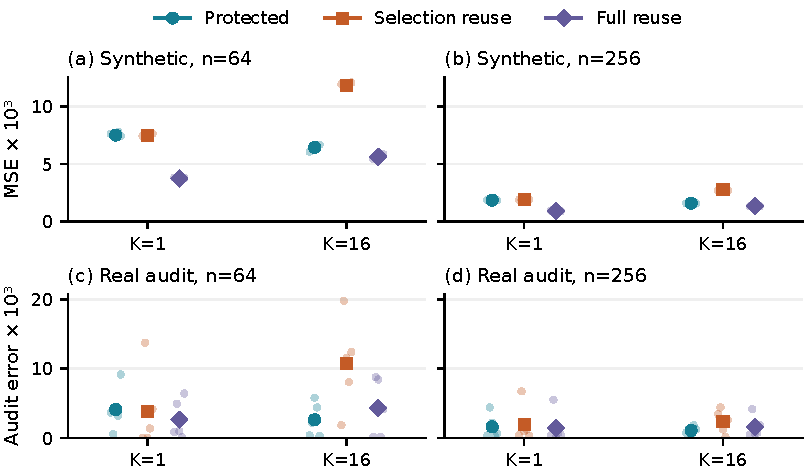
\includegraphics[width=\textwidth]{figures/reporting_error_comparison.pdf}
\caption{Error depends on selection multiplicity, question budget, and reference. Large markers show means over evaluation seeds; small dots show each seed, horizontally offset for visibility. Synthetic values average regimes and replicates; real values are discrepancies to finite audits. Vertical scales are shared within each row, not across evidence families. Protected versus selection reuse holds the prompt fixed; full reuse may select a different prompt. Values are multiplied by $10^3$.}
% @evidence[[analysis/condition_results.csv]]
\label{fig:errors}
\end{figure}

Table~\ref{tab:main} keeps all comparators visible. Full reuse has lower mean error than protected reporting in \emph{every synthetic condition}, including both sixteen-prompt settings. Thus reducing selection optimism need not minimize MSE: reusing all questions trades some selection bias for a larger assessment sample, and also selects a potentially different system. The fixed and random comparators often have still lower MSE. This does not establish higher selected-prompt accuracy, because each comparator is assessed against its own reference. A good estimate of a weaker prompt is not an improved prompt.
% @evidence[[analysis/summary.json#/condition_means]]

\begin{table}[t]
\caption{Mean error $\times10^3$ across seeds. Synthetic entries use known truth; real entries use finite audit accuracy. Reuse means same-winner selection-score reuse; Full selects and reports on all questions; Half is the alternative protected split. Fixed and Random also use all questions. Different selectors can have different targets, so this is not a ranking of answer accuracy.}
\label{tab:main}
\centering\small
\setlength{\tabcolsep}{4pt}
% @evidence[[paper_data.json#/final_evaluation/evaluation_evidence/episodes]]
\begin{tabular}{llrrrrrr}\toprule
Setting & $(n,K)$ & Protected & Reuse & Full & Half & Fixed & Random\\\midrule
Synthetic & (64,1) & 7.514 & 7.459 & 3.741 & 7.455 & 3.741 & 3.741\\
Synthetic & (64,16) & 6.439 & 11.858 & 5.635 & 6.480 & 3.776 & 3.458\\
Synthetic & (256,1) & 1.850 & 1.889 & 0.922 & 1.890 & 0.922 & 0.922\\
Synthetic & (256,16) & 1.586 & 2.768 & 1.359 & 1.572 & 0.948 & 0.857\\
Real audit & (64,1) & 4.098 & 3.854 & 2.657 & 3.732 & 2.657 & 2.657\\
Real audit & (64,16) & 2.620 & 10.725 & 4.329 & 1.170 & 2.657 & 3.793\\
Real audit & (256,1) & 1.603 & 1.926 & 1.432 & 1.536 & 1.432 & 1.432\\
Real audit & (256,16) & 1.089 & 2.359 & 1.571 & 1.542 & 1.432 & 1.783\\
\bottomrule\end{tabular}

\end{table}

The single-prompt conditions expose the cost without multiplicity. At $n=64$, protected MSE is $0.007514$ in simulation versus $0.003741$ for full reuse; the real audit-reference errors are $0.004098$ versus $0.002657$. With no prompt selection to protect against, withholding half the assessment observations has no selection-bias benefit. The smaller differences between protected reporting and selection reuse in these conditions instead reflect finite-sample behavior of two complementary halves. The observed negative comparison is important: the method is not a generic variance-reduction device.
% @evidence[[analysis/summary.json#/condition_means/S64K1]]
% @evidence[[analysis/summary.json#/condition_means/R64K1]]

The supplied equal-weight aggregate error is $0.003350$ for protected reporting, compared with $0.005355$ for same-winner reuse, $0.002706$ for full reuse, and $0.002196$ for the fixed prompt. We report this summary for completeness, not as a population risk across unrelated synthetic and real conditions. Its ordering preserves the central conclusion: protection helps against the matched reuse comparator, but does not dominate all alternatives.
% @evidence[[paper_data.json#/final_evaluation/metrics/report_mse]]
% @evidence[[paper_data.json#/final_evaluation/metrics/reuse_mse]]
% @evidence[[paper_data.json#/final_evaluation/metrics/full_budget_naive_mse]]
% @evidence[[paper_data.json#/final_evaluation/metrics/fixed_prompt_mse]]

\subsection{Dependence Modulates Optimism, Not the Meaning of Protection}
The synthetic regimes make the reporting mechanism easier to interpret than the overall error alone. Table~\ref{tab:regimes} averages the sixteen-prompt conditions across both question budgets. Equal-accuracy prompts under low coupling exhibit $10.639$ percentage points of mean selection optimism; high coupling lowers this to $2.776$ points. The corresponding values for graded accuracies are $5.599$ and $1.768$ points. Less independent variation among prompt outcomes leaves less noise for the maximization to exploit. This interpretation is restricted to the specified joint outcome construction, not a quantitative dependence law for real prompts.
% @evidence[[analysis/summary.json#/regime_means]]

\begin{table}[t]
\centering\small
\caption{Known-truth diagnostic means for $K=16$, equally weighting seeds and $n=64,256$. Bias is protected-report minus truth; optimism is selection reuse minus truth. Coupling is the shared-branch probability in Equation~\ref{eq:synthetic}. Coverage and interval width refer to the protected Wilson interval. Percentage points (pp) are used only for the two signed errors.}
\label{tab:regimes}
% @evidence[[paper_data.json#/final_evaluation/evaluation_evidence/episodes]]
\begin{tabular}{llrrrr}\toprule
Truth & Coupling & Bias (pp) & Optimism (pp) & Coverage & Width\\\midrule
Equal & Low & 0.001 & 10.639 & 0.953 & 0.242\\
Equal & High & 0.003 & 2.776 & 0.954 & 0.242\\
Graded & Low & 0.028 & 5.599 & 0.950 & 0.210\\
Graded & High & 0.069 & 1.768 & 0.953 & 0.205\\
\bottomrule\end{tabular}

\end{table}

Protected signed bias is much smaller than reuse optimism in these regime averages, but that is not the same as vanishing uncertainty. At $K=16$, mean Wilson coverage is $0.95195$ for $n=64$ and $0.95264$ for $n=256$; mean interval width is $0.29608$ and $0.15287$. These are measured repeated-simulation properties close to the nominal level under the implemented distribution. They neither prove exact finite-sample coverage nor establish coverage under adaptive prompt generation, subject dependence, or another benchmark distribution.
% @evidence[[analysis/summary.json#/condition_means/S64K16]]
% @evidence[[analysis/summary.json#/condition_means/S256K16]]

The alternative half split further cautions against overattribution. Its real $n=64,K=16$ error is $0.001170$, below the randomized split's $0.002620$; at $n=256,K=16$ the ordering reverses, with $0.001542$ versus $0.001089$. Both designs protect a report set, but use different row allocations and can choose different prompts. The comparison supports sensitivity to the realized split, not a claim that a particular randomization procedure is intrinsically better. No successful controlled comparison of alternative allocation fractions or subject-balancing rules is available.
% @evidence[[analysis/summary.json#/condition_means/R64K16]]
% @evidence[[analysis/summary.json#/condition_means/R256K16]]

\subsection{Finite-Audit Evidence Does Not Establish an Accuracy Gain}
For the real sixteen-prompt conditions, average audit accuracy of the selected prompt is $12.031\%$ at $n=64$ and $11.641\%$ at $n=256$. These modest values concern this small model with constrained direct answers; they do not characterize larger LLMs or alternative decoding procedures. The report and reuse conditions share that accuracy by construction. Their estimation-error contrast cannot establish that protection produces a better system.
% @evidence[[analysis/summary.json#/condition_means/R64K16/selected_accuracy]]
% @evidence[[analysis/summary.json#/condition_means/R256K16/selected_accuracy]]

\begin{figure}[t]
\centering
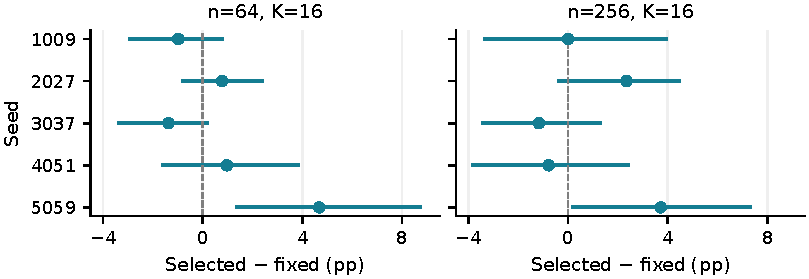
\includegraphics[width=\textwidth]{figures/real_audit_accuracy_difference.pdf}
\caption{Selected-minus-fixed audit accuracy for each seed at $K=16$. Points use paired outcomes on the same audit; lines are the recorded subject-bootstrap percentile intervals. Zero is included in eight of the ten intervals. Both positive exclusions occur for seed $5059$, not independent benchmark replications. Intervals are descriptive, not simultaneous, and do not quantify population coverage of the reporting rule.}
% @evidence[[analysis/summary.json#/audit_differences]]
\label{fig:audit}
\end{figure}

Figure~\ref{fig:audit} asks the separate question of whether the selected prompt is more accurate than the default prompt. Eight of ten recorded intervals include zero; the two positive exclusions both belong to seed $5059$. This is not evidence of a consistent accuracy gain, and the overlapping question pools preclude reading those exclusions as two independent confirmations. For $K=1$ the selected and default prompts coincide, giving identically zero paired differences. These controls help distinguish honest reporting from improved selection.
% @evidence[[analysis/summary.json#/audit_differences]]

All ten real sixteen-prompt Wilson intervals contain their respective finite-audit accuracies. Across the remaining real conditions, one of the single-prompt intervals fails to contain the audit reference. Neither observation estimates 95\% population coverage with meaningful precision: the number of realized settings is small, the audit accuracy is noisy, and settings share data. Likewise, a lower audit-reference error may reflect both estimation quality and the particular audit realization. We therefore keep the real findings at the level of measured audit agreement.
% @evidence[[analysis/summary.json#/condition_means]]
% @evidence[[analysis/condition_results.csv]]

\section{Discussion and Limitations}
\paragraph{What a reported number should identify.}
The evidence supports documenting three objects together: the selected configuration, the observations used for selection and reporting, and the target against which reliability is assessed. A reused selection score describes an observation after maximization; a protected score describes the same configuration using other observations. A full-budget score may describe another configuration entirely. An interval around any of these numbers does not, by itself, settle which comparison is appropriate. This is why the strongest matched reporting comparison and the strongest error counterexamples both belong in the main results.

\paragraph{What the study does not isolate.}
The same-winner contrast isolates the reporting-row substitution within a fixed split. It does not isolate every effect of an end-to-end optimization pipeline. Fixed versus searched prompts, randomized versus alternative splits, and full-budget versus half-budget selection change multiple quantities. The bank is frozen, with no outcome-dependent prompt generation, repeated release of holdout feedback, or independent assessment of a learned search policy. Unmeasured allocation rules and unavailable ablations cannot support component-level conclusions. No result demonstrates that a report set remains protected after repeated human or automated inspection.

\paragraph{Question populations and dependence.}
The known-truth construction uses independent question rows and specified prompt dependence. Public benchmark questions need not follow that model. The real audit is held apart from selection within its condition, but it is a finite sample from a shared public pool. Overlap across seeds, unmeasured difficulty structure, possible training contamination, and semantic duplication beyond normalization all limit population interpretation. The subject bootstrap preserves paired within-question comparisons but has few draws and no demonstrated calibration here. Neither the bootstrap intervals nor the aggregate containment indicator should be advertised as a validated deployment guarantee.

\paragraph{Decision reliability is a separate target.}
The evaluation also records whether the protected-report comparison with the all-question default score has the opposite strict sign to the reference accuracy comparison. In notation, it checks
$\mathbf{1}\{(\widehat p_{\rm protect}-\overline X_{\cdot1})(a_{\widehat j}-a_1)<0\}$,
where $a$ denotes known truth in simulation or observed audit accuracy for real questions. Ties do not count as disagreements; they remain in the averaging denominator. In the real sixteen-prompt conditions, this diagnostic is one in four of five seeds at $n=64$ and one of five at $n=256$. Thus a lower reporting MSE does not ensure a stable directional comparison on the observed samples. However, the diagnostic mixes a protected selected-prompt report with an all-question fixed-prompt report, and its real reference is itself noisy. It is not the probability that a naive superiority claim is overturned, does not compare two independently trained systems, and supplies no population decision-error guarantee. Reporting the exact comparison is more informative than calling every sign change a failed optimization.
% @evidence[[analysis/summary.json#/condition_means/R64K16/decision_reversal_rate]]
% @evidence[[analysis/summary.json#/condition_means/R256K16/decision_reversal_rate]]
% @evidence[[source_evidence/evaluate_final.py#L779]]

\paragraph{Implementation and qualification boundaries.}
Evaluator-owned controls check constant outcomes, copied prompt columns, a deliberately contaminated report, effective input permutation, and reset/replay. The deliberately contaminated control records failed independence, as intended. The supplied aggregate control-failure and replay-discrepancy values are zero. Those facts support specific implementation checks, not full statistical validity. The final record marks qualification successful, while candidate diagnostic trust is explicitly unverified; missing gate-level detail is not inferred from the retained metrics. The inspected evaluator file matches its recorded digest, but differently scoped source-tree digests do not establish an undocumented stronger identity.
% @evidence[[paper_data.json#/final_evaluation/metrics/control_failure_rate]]
% @evidence[[paper_data.json#/final_evaluation/metrics/replay_discrepancy]]
% @evidence[[paper_data.json#/final_evaluation/outcome]]
% @evidence[[source_evidence/evaluate_final.py#L785]]

\paragraph{Resources and reproducibility.}
The recorded seed evaluations take approximately $31$--$51$ minutes each, totaling $3.40$ hours when their durations are summed. This is a sum of reported wall durations, not measured CPU-hours, inference-only time, or an end-to-end budget accounting. GPU use, energy, and realized token totals are not supplied. The inference implementation is CPU based and caches predictions, so multiplying conditions by question counts would overstate distinct model calls. Supplementary Information and the accompanying reproduction guide identify versions, commands, seeds, and the script producing every quantitative table and figure. No new model inference or simulation was run to write this paper.
% @evidence[[analysis/summary.json#/episode_durations_seconds]]
% @evidence[[analysis/summary.json#/duration_sum_seconds]]
% @evidence[[source_evidence/evaluate_final.py#L574]]

\section{Conclusion}
Protected reporting answers a narrower question than whether automatic prompt optimization works: it concerns how accurately a selected system's performance is described. In the evaluated sixteen-prompt settings, a held-apart half sample yields lower mean error than reusing the same prompt's selection score. Known-truth simulations show the accompanying reduction in signed optimism, and real inference provides a finite-audit check. Neither establishes that protected reporting improves selected-prompt accuracy or dominates alternative uses of the available observations.

The negative comparisons matter equally. Full-budget reuse has lower mean error in every synthetic condition, fixed-prompt reporting can be easier to estimate, and two protected splits can differ substantially on a realized benchmark sample. Thus reliability cannot be summarized by naming an estimator without its target and observation budget. The practical implication is to disclose selection and reporting data roles, retain budget-aware comparators, and distinguish population-error evidence from audit agreement. The current evidence supports that bounded reporting discipline, not a general guarantee for adaptive optimization or deployment on new question populations.
% @evidence[[analysis/summary.json#/condition_means]]

\clearpage
\bibliography{references}
\bibliographystyle{iclr2026_conference}

\clearpage
\appendix
\section{Supplementary Information}
\subsection{Complete Seed-Level Results}
Table~\ref{tab:seed} gives every recorded condition. Error values are multiplied by $10^3$; target accuracy, coverage, and interval width remain on the unit scale. Synthetic targets and diagnostics average four regimes with $1024$ replicates each. A real row has a single audit-reference error and a binary containment indicator, so a value of one is not an estimate of certain population coverage. The machine-readable \texttt{analysis/condition\_results.csv} additionally includes all six comparator errors, signed errors, and recorded diagnostics. \texttt{analysis/regime\_results.csv} preserves the full regime-level metrics and supplied report-MSE standard errors; these marginal standard errors are not used as errors for paired method differences. \texttt{analysis/summary.json} supplies equal-weight condition and regime means without additional scientific evaluations.
% @evidence[[paper_data.json#/final_evaluation/evaluation_evidence/episodes]]
\begin{center}
\small
\captionof{table}{All seed-level conditions. Report and Reuse are squared-error metrics $\times10^3$. Target is selected-prompt known accuracy for synthetic rows and finite-audit accuracy for real rows. Cov. denotes population coverage only for synthetic rows; for real rows it denotes audit containment.}
\label{tab:seed}
% @evidence[[paper_data.json#/final_evaluation/evaluation_evidence/episodes]]
\begin{longtable}{rrlrrrrrr}\toprule
Seed & $n$ & Setting & $K$ & Report & Reuse & Target & Cov. & Width\\\midrule\endhead
1009 & 64 & Synth. & 1 & 7.6179 & 7.4306 & 0.5000 & 0.9519 & 0.3169\\
1009 & 64 & Synth. & 16 & 6.0695 & 11.9401 & 0.6842 & 0.9597 & 0.2964\\
1009 & 256 & Synth. & 1 & 1.8620 & 1.9005 & 0.5000 & 0.9536 & 0.1667\\
1009 & 256 & Synth. & 16 & 1.5774 & 2.7214 & 0.6951 & 0.9517 & 0.1528\\
1009 & 64 & Real & 1 & 3.6659 & 0.0038 & 0.1230 & 1.0000 & 0.1842\\
1009 & 64 & Real & 16 & 0.3815 & 1.8463 & 0.1133 & 1.0000 & 0.2098\\
1009 & 256 & Real & 1 & 0.3815 & 0.3815 & 0.1133 & 1.0000 & 0.1178\\
1009 & 256 & Real & 16 & 0.7477 & 3.4332 & 0.1133 & 1.0000 & 0.0987\\
2027 & 64 & Synth. & 1 & 7.4230 & 7.3855 & 0.5000 & 0.9531 & 0.3168\\
2027 & 64 & Synth. & 16 & 6.3961 & 11.7112 & 0.6843 & 0.9473 & 0.2962\\
2027 & 256 & Synth. & 1 & 1.8362 & 1.8925 & 0.5000 & 0.9570 & 0.1667\\
2027 & 256 & Synth. & 16 & 1.6153 & 2.8066 & 0.6947 & 0.9514 & 0.1529\\
2027 & 64 & Real & 1 & 0.5493 & 13.7329 & 0.1016 & 1.0000 & 0.2310\\
2027 & 64 & Real & 16 & 2.1973 & 19.7754 & 0.1094 & 1.0000 & 0.2489\\
2027 & 256 & Real & 1 & 4.4098 & 6.7291 & 0.0820 & 0.0000 & 0.1231\\
2027 & 256 & Real & 16 & 1.2360 & 4.4098 & 0.1055 & 1.0000 & 0.1205\\
3037 & 64 & Synth. & 1 & 7.3059 & 7.5013 & 0.5000 & 0.9578 & 0.3168\\
3037 & 64 & Synth. & 16 & 6.6277 & 11.7846 & 0.6846 & 0.9500 & 0.2954\\
3037 & 256 & Synth. & 1 & 1.8511 & 1.9148 & 0.5000 & 0.9534 & 0.1667\\
3037 & 256 & Synth. & 16 & 1.5947 & 2.7543 & 0.6953 & 0.9519 & 0.1529\\
3037 & 64 & Real & 1 & 3.9062 & 0.0000 & 0.1250 & 1.0000 & 0.2642\\
3037 & 64 & Real & 16 & 5.8022 & 11.5395 & 0.1113 & 1.0000 & 0.2642\\
3037 & 256 & Real & 1 & 2.1973 & 0.9766 & 0.1172 & 1.0000 & 0.1279\\
3037 & 256 & Real & 16 & 0.3815 & 1.2360 & 0.1055 & 1.0000 & 0.1150\\
4051 & 64 & Synth. & 1 & 7.7847 & 7.3543 & 0.5000 & 0.9502 & 0.3166\\
4051 & 64 & Synth. & 16 & 6.4329 & 11.7671 & 0.6835 & 0.9541 & 0.2965\\
4051 & 256 & Synth. & 1 & 1.8643 & 1.8607 & 0.5000 & 0.9558 & 0.1667\\
4051 & 256 & Synth. & 16 & 1.5659 & 2.8667 & 0.6950 & 0.9558 & 0.1529\\
4051 & 64 & Real & 1 & 3.2082 & 1.3771 & 0.1191 & 1.0000 & 0.1842\\
4051 & 64 & Real & 16 & 4.4098 & 8.0719 & 0.1289 & 1.0000 & 0.1842\\
4051 & 256 & Real & 1 & 0.3815 & 1.2360 & 0.1367 & 1.0000 & 0.1120\\
4051 & 256 & Real & 16 & 1.8463 & 0.1373 & 0.1289 & 1.0000 & 0.0987\\
5059 & 64 & Synth. & 1 & 7.4386 & 7.6242 & 0.5000 & 0.9546 & 0.3167\\
5059 & 64 & Synth. & 16 & 6.6704 & 12.0853 & 0.6830 & 0.9487 & 0.2958\\
5059 & 256 & Synth. & 1 & 1.8363 & 1.8774 & 0.5000 & 0.9561 & 0.1667\\
5059 & 256 & Synth. & 16 & 1.5746 & 2.6933 & 0.6950 & 0.9524 & 0.1529\\
5059 & 64 & Real & 1 & 9.1591 & 4.1542 & 0.0918 & 1.0000 & 0.2642\\
5059 & 64 & Real & 16 & 0.3090 & 12.3940 & 0.1387 & 1.0000 & 0.2489\\
5059 & 256 & Real & 1 & 0.6447 & 0.3090 & 0.0918 & 1.0000 & 0.1120\\
5059 & 256 & Real & 16 & 1.2360 & 2.5787 & 0.1289 & 1.0000 & 0.1279\\
\bottomrule\end{longtable}
\end{center}

\subsection{Partition, Estimand, and Interval Details}
The default instruction is: ``Answer the multiple-choice question. Return only the correct option letter A through J.'' The remaining bank entries are fixed paraphrases requesting a single capital letter without explanation. The complete bank is inspectable in \texttt{source\_evidence/downstream/}\texttt{program/src/program.py}, lines 55--76. The same file's reset and update handlers, lines 78--102, implement the seeded shuffle, half partition, uniform weights, and fixed priority. The preserved baseline and studied policy files are byte-identical; they are not counted as distinct scientific comparators.
% @evidence[[source_evidence/downstream/program/src/program.py#L70]]
% @evidence[[source_evidence/downstream/baseline/src/program.py]]

For report mean $\widehat p$, count $m=|R|$, and $z=1.959963984540054$, the implemented Wilson interval has center and half-width
\begin{equation}
 C=\frac{\widehat p+z^2/(2m)}{1+z^2/m},\qquad
 H=\frac{z\sqrt{\widehat p(1-\widehat p)/m+z^2/(4m^2)}}{1+z^2/m}.
\end{equation}
The returned interval is $[C-H,C+H]$. Its use here is a specified conventional construction, not a claim of exact coverage. The selected prompt is evaluated on $m$ report rows regardless of how many prompts were considered. Comparators other than same-winner reuse may have another selected prompt, so their squared errors substitute their own corresponding reference accuracy.
% @evidence[[source_evidence/evaluate_final.py#L746]]

For audit subject bootstrap intervals, per-question differences are selected-prompt accuracy minus default-prompt accuracy. The evaluator samples the list of observed subjects with replacement and concatenates all question differences from every sampled subject, including multiplicities. The resulting mean is question-weighted within that resampled collection, not an equal-weight average of subject means. It takes the $0.025$ and $0.975$ empirical quantiles of $200$ draws using generator seed equal to the evaluation seed plus $76531$. This construction holds the observed selected prompt fixed; it does not repeat selection inside each bootstrap draw.
% @evidence[[source_evidence/evaluate_final.py#L987]]

\subsection{Diagnostic Controls and Evidence Boundaries}
The constant control sets all entries to zero and requires tie priority to be respected. The copied-column control repeats the default column across prompts and again checks tie priority. Neither is an empirical test of generalization. The contaminated-report control intentionally uses selection rows for reporting and verifies that reused and reported scores coincide; its independence flag is false. This is an expected detection, not a failure of the intended disjoint partition. Synthetic permutation rolls outcome rows; the real permutation changes answer assignments and checks that the change is nonvacuous. These controls do not measure every possible leakage mechanism.
% @evidence[[source_evidence/evaluate_final.py#L785]]
% @evidence[[source_evidence/evaluate_final.py#L976]]

The final record independently reports completion and successful qualification. No final qualification failure is present. The absence of a scored replacement during development is separate: there are zero scored and three unscored alternative evaluations. Timeout records do not reveal those alternatives' scientific performance or identify a causal reason for missing scores. We consequently make no comparative claim about their allocation policies. Search-scope scores are neither final-scope measurements nor answer accuracies and are not used in the paper's quantitative comparisons.
% @evidence[[paper_data.json#/final_evaluation/status]]
% @evidence[[paper_data.json#/final_evaluation/outcome]]
% @evidence[[paper_data.json#/downstream_study/attempt_counts]]

The local evaluator digest equals the recorded evaluator digest. This links the inspected estimator, inference, and diagnostic definitions to a named evaluator file. It does not establish equality between every differently scoped source tree in the provenance record. Likewise, an earlier audit verdict or a file hash is not the substantive evidence for a detailed implementation claim; the readable source locations above provide that evidence. Detailed gate explanations absent from the supplied record remain unknown, and candidate-origin diagnostic annotations remain unverified.
% @evidence[[paper_data.json#/final_evaluation/evaluator_sha256]]
% @evidence[[source_evidence/evaluate_final.py]]

\subsection{Reproducibility and Resource Accounting}
The fixed model revision is \texttt{12fd25f77366fa6b3b4b768ec3050bf629380bac}; MMLU-Pro is fixed at revision \texttt{b189ec765aa7ed75c8acfea42df31fdae71f97be}. The retained real pool has $4096$ examples. Normalization uses Unicode NFKC and collapses whitespace; option-content matching sorts normalized options. The split manifest records $11711$ unique groups and allocation seed $732091$. These describe dataset preparation, not additional measured performance. Data may have appeared in pretraining.
% @evidence[[source_evidence/resources/runtime_manifest.json]]
% @evidence[[source_evidence/resources/split_manifest.json]]
% @evidence[[source_evidence/resources/examples.json]]

The supplied dependency specification pins NumPy 2.2.6, PyArrow 19.0.1, PyTorch 2.6.0, Transformers 4.51.3, Safetensors 0.5.3, SciPy 1.15.3, and Matplotlib 3.10.3. The runtime manifest identifies CPython 3.12 on Linux x86\_64, CPU float32 inference and float64 statistics. The answer worker uses two tensor threads and one interoperation thread. These are the supplied environment specification and inspected settings; a separately retained package inventory proving every version actually loaded is unavailable. The paper-artifact environment is recorded separately in the reproduction guide.
% @evidence[[source_evidence/requirements.txt]]
% @evidence[[source_evidence/resources/runtime_manifest.json]]
% @evidence[[source_evidence/evaluate_final.py#L574]]

To regenerate manuscript analyses without model calls, run \texttt{python build\_artifacts.py}. It reads the immutable final record and produces both quantitative figures as PDF and 300-DPI PNG, the main comparison table, the regime table, the complete seed table, and their evidence sidecars. The retained overview is a title-only placeholder because rendering failed; the build script preserves any existing overview image. The exact final-evaluation entrypoint, resource acquisition details, and validation commands are in \texttt{REPRODUCIBILITY.md}. Evaluation commands there describe future reproduction, not additional executions during manuscript preparation. Predicted reproduction time is uncertain because the recorded durations include shared caching and orchestration overhead; the measured duration sum is the only supplied wall-time accounting.
% @evidence[[build_artifacts.py]]
% @evidence[[figures/reporting_overview.prompts.json]]
% @evidence[[concept_figure_run.log]]
% @evidence[[analysis/summary.json#/duration_sum_seconds]]

References were consulted through fixed original arXiv abstracts, original journal pages, or original publisher-deposited abstracts and bibliographic records, as individually recorded in \texttt{references\_provenance.json}. No citation graph or broad topical discovery was used. Full-text reading is not claimed when only an abstract was consulted. No known encounter with the prohibited study occurred. The official ICLR 2026 style and bibliography style were obtained directly from the ICLR template repository, rather than relabeling a template for another year.

\subsection{LLM Usage}
LLM-based research assistance contributed to proposal generation, implementation editing, reference planning, narrative selection, plotting code, manuscript drafting, and evidence checking. The research assistance is distinct from the evaluated answer generator, SmolLM2-135M-Instruct. Its role in evaluation is limited to producing the constrained answer letters described in the method. The writing assistant inspected the supplied results and source, generated deterministic summaries and figures, and validated the manuscript; it did not run new scientific inference or simulations for this paper. Literature retrieval used fixed identifiers for permitted originals. No unrecorded human validation, external audit, or independent replication is asserted.

\end{document}
